%% This is file `elsarticle-template-2-harv.tex',
%%
%% Copyright 2009 Elsevier Ltd
%%
%% This file is part of the 'Elsarticle Bundle'.
%% ---------------------------------------------
%%
%% It may be distributed under the conditions of the LaTeX Project Public
%% License, either version 1.2 of this license or (at your option) any
%% later version.  The latest version of this license is in
%%    http://www.latex-project.org/lppl.txt
%% and version 1.2 or later is part of all distributions of LaTeX
%% version 1999/12/01 or later.
%%
%% The list of all files belonging to the 'Elsarticle Bundle' is
%% given in the file `manifest.txt'.
%%
%% Template article for Elsevier's document class `elsarticle'
%% with harvard style bibliographic references
%%
%% $Id: elsarticle-template-2-harv.tex 155 2009-10-08 05:35:05Z rishi $
%% $URL: http://lenova.river-valley.com/svn/elsbst/trunk/elsarticle-template-2-harv.tex $
%%

%%\documentclass[preprint,authoryear,12pt]{elsarticle}

%% Use the option review to obtain double line spacing
%% \documentclass[authoryear,preprint,review,12pt]{elsarticle}

%% Use the options 1p,twocolumn; 3p; 3p,twocolumn; 5p; or 5p,twocolumn
%% for a journal layout:

%% Astronomy & Computing uses 5p
%% \documentclass[final,authoryear,5p,times]{elsarticle}
\documentclass[final,authoryear,5p,times,twocolumn]{elsarticle}

%% if you use PostScript figures in your article
%% use the graphics package for simple commands
%% \usepackage{graphics}
%% or use the graphicx package for more complicated commands
\usepackage{graphicx}
%% or use the epsfig package if you prefer to use the old commands
%% \usepackage{epsfig}

%% The amssymb package provides various useful mathematical symbols
\usepackage{amssymb}
%% The amsthm package provides extended theorem environments
%% \usepackage{amsthm}

\usepackage[pdftex,pdfpagemode={UseOutlines},bookmarks,bookmarksopen,colorlinks,linkcolor={blue},citecolor={green},urlcolor={red}]{hyperref}
\usepackage{hypernat}

%% The lineno packages adds line numbers. Start line numbering with
%% \begin{linenumbers}, end it with \end{linenumbers}. Or switch it on
%% for the whole article with \linenumbers after \end{frontmatter}.
%% \usepackage{lineno}

%% natbib.sty is loaded by default. However, natbib options can be
%% provided with \biboptions{...} command. Following options are
%% valid:

%%   round  -  round parentheses are used (default)
%%   square -  square brackets are used   [option]
%%   curly  -  curly braces are used      {option}
%%   angle  -  angle brackets are used    <option>
%%   semicolon  -  multiple citations separated by semi-colon (default)
%%   colon  - same as semicolon, an earlier confusion
%%   comma  -  separated by comma
%%   authoryear - selects author-year citations (default)
%%   numbers-  selects numerical citations
%%   super  -  numerical citations as superscripts
%%   sort   -  sorts multiple citations according to order in ref. list
%%   sort&compress   -  like sort, but also compresses numerical citations
%%   compress - compresses without sorting
%%   longnamesfirst  -  makes first citation full author list
%%
%% \biboptions{longnamesfirst,comma}

% \biboptions{}

\journal{Astronomy \& Computing}

%% Make single quotes look right in verbatim mode
\usepackage{upquote}

\usepackage{upgreek}

\begin{document}

\begin{frontmatter}

%% Title, authors and addresses

%% use the tnoteref command within \title for footnotes;
%% use the tnotetext command for the associated footnote;
%% use the fnref command within \author or \address for footnotes;
%% use the fntext command for the associated footnote;
%% use the corref command within \author for corresponding author footnotes;
%% use the cortext command for the associated footnote;
%% use the ead command for the email address,
%% and the form \ead[url] for the home page:
%%
%% \title{Title\tnoteref{label1}}
%% \tnotetext[label1]{}
%% \author{Name\corref{cor1}\fnref{label2}}
%% \ead{email address}
%% \ead[url]{home page}
%% \fntext[label2]{}
%% \cortext[cor1]{}
%% \address{Address\fnref{label3}}
%% \fntext[label3]{}

\title{The Future of Astronomical Data Formats II. Learning from 25
  years of the extensible \emph{N}-Dimensional Data Format}

%% use optional labels to link authors explicitly to addresses:
%% \author[label1,label2]{<author name>}
%% \address[label1]{<address>}
%% \address[label2]{<address>}

\author[cornell]{Tim Jenness\corref{cor1}}
\ead{tjenness@cornell.edu}
\author[jac]{David S. Berry}
\author[jac]{Malcolm J.\ Currie}
\author[durham]{Peter W.\ Draper}
\author[noao]{Frossie Economou}
\author[glasgow]{Norman Gray}
\author[ral]{Brian McIlwrath}
\author[aao]{Keith Shortridge}
\author[bristol]{Mark B.\ Taylor}
\author[ral]{Patrick T.\ Wallace}
\author[ral]{Rodney F.\ Warren-Smith}

\cortext[cor1]{Corresponding author}

\address[cornell]{Department of Astronomy, Cornell University, Ithaca,
  NY 14853, USA}
\address[jac]{Joint Astronomy Centre, 660 N.\ A`oh\=ok\=u Place, Hilo, HI
  96720, USA}
\address[durham]{Department of Physics, Institute for Computational Cosmology, University of Durham, South Road, Durham DH1 3LE, UK}
\address[noao]{National Optical Astronomy
  Observatory, 950 N Cherry Ave, Tucson, AZ 85719, USA}
\address[glasgow]{SUPA School of Physics \& Astronomy, University of Glasgow, Glasgow G12 8QQ, UK}
\address[ral]{RAL Space, STFC Rutherford Appleton Laboratory, Harwell Oxford, Didcot, Oxfordshire OX11 0QX, UK}
\address[aao]{Australian Astronomical Observatory, 105 Delhi Rd, North
Ryde, NSW 2113, Australia}
\address[bristol]{H.\ H.\ Wills Physics Laboratory, Bristol University, Tyndall Avenue, Bristol, UK}

\begin{abstract}
%% Text of abstract

The extensible \emph{N}-dimensional Data Format (NDF) was designed and
developed in the late 1980s to provide a data model suitable for use
in a variety of astronomy data processing applications supported by
Starlink. Starlink applications were used extensively, primarily in
the UK astronomical community, and form the basis of a number of
advanced data reduction pipelines today. This paper provides an
overview of the historical drivers for the development of NDF and the
lessons learned from using a defined hierarchical data model for many
years in data reduction software, data pipelines and in data
acquisition systems.

\end{abstract}

\begin{keyword}
%% keywords here, in the form: keyword \sep keyword

%% MSC codes here, in the form: \MSC code \sep code
%% or \MSC[2008] code \sep code (2000 is the default)

data formats \sep
Starlink

\end{keyword}

\end{frontmatter}

% \linenumbers

%% Journal abbreviations
\newcommand{\mnras}{Mon Not R Astron Soc}
\newcommand{\aap}{Astron Astrophys}
\newcommand{\aaps}{Astron Astrophys Supp}
\newcommand{\pasp}{Pub Astron Soc Pacific}
\newcommand{\apj}{Astrophys J}
\newcommand{\apjs}{Astrophys J Supp}
\newcommand{\qjras}{Quart J R Astron Soc}
\newcommand{\an}{Astron.\ Nach.}
\newcommand{\ijimw}{Int.\ J.\ Infrared \& Millimeter Waves}
\newcommand{\procspie}{Proc.\ SPIE}
\newcommand{\aspconf}{ASP Conf. Ser.}

%% Applications

\newcommand{\KAPPA}{\textsc{kappa}}
\newcommand{\gaia}{\textsc{gaia}}
\newcommand{\ccdpack}{\textsc{ccdpack}}
\newcommand{\smurf}{\textsc{smurf}}
\newcommand{\asterix}{\textsc{asterix}}
\newcommand{\specdre}{\textsc{specdre}}
\newcommand{\iras}{\textsc{iras90}}
\newcommand{\treeview}{\textsc{treeview}}
\newcommand{\splat}{\textsc{splat}}

%% Links
\newcommand{\ascl}[1]{\href{http://www.ascl.net/#1}{ascl:#1}}

%% main text
\section{Introduction}
\label{sec:intro}

There is a renewed interest in file format choices for astronomy
with discussions on the future of FITS
\citep{P90_adassxxiii,2014Thomas}, projects adopting or considering
HDF5 \citep{2012ASPC..461..283A,P10_adassxxiii} and investigations into
non-scientific formats such as JPEG2000 \citep{2014Kitaeff}. These
discussions have provided an opportunity to consider existing
astronomy file formats that are not as widely known in the community
as FITS. Here we discuss the extensible \emph{N}-Dimensional
Data Format (NDF) developed by the Starlink Project
\citep{1982MmSAI..53...55T,2000ASSL..250...93W} in the late 1980s
\citep{1988STARB...2...11C,SGP38} to bring order to the proliferation
of data models that were being adopted by applications using the Starlink
hierarchical file format.

In Sec.\ \ref{sec:hds} we discuss the genesis and features of the Starlink
file format, then in Sec.\ \ref{sec:chaos} we provide examples of data
models developed in the mid-1980s. The NDF data model itself is
discussed in Sec.\ \ref{sec:ndf} and its usage in data acquisition
system is covered in Sec.\ \ref{sec:daq}. We finish in Sec.\
\ref{sec:lessons} by discussing the positive lessons learned from
developing NDF and the areas where NDF could be improved, expanding on
some earlier work \citep{P91_adassxxiii}.

\section{Hierarchical Data System}
\label{sec:hds}

The Starlink Project, created in 1980
\citep{1980IrAJ...14..197E,1982MmSAI..53...55T}, was set up
primarily to provide data reduction software and facilities to United
Kingdom astronomers. FITS
\citep{1979ipia.coll..445W,1981A&AS...44..363W} had recently been
developed and was adopted as a tape interchange format but there was a
requirement for a file format optimized for data reduction that all
Starlink applications could understand. Files
needed to be written to and read from efficiently with an emphasis on the
ability to group and modify related information
\citep{1981STARENT4}. This was many years before the NCSA developed
the Hierarchical Data Format \citep{HDF1,Folk2010} and it was decided
to develop a new file format. The resulting Starlink Data
System\footnote{from which the file extension of \texttt{.sdf}, for
  Starlink Data File, was chosen.} was first proposed in 1981 with the
first version being released in 1982 \citep[see
e.g.][]{1982QJRAS..23..485D,1991STARB...8....2L}. In 1983 the name was
changed to the Hierarchical Data System (HDS) to make the file format
benefits more explicit. HDS itself was in common usage within Starlink by 1986
\citep{1986BICDS..30...13L}. It was originally written in the BLISS
programming language on a VAX/VMS system and later rewritten in C and
ported to Unix.

Some key features of the HDS design are as follows.
\begin{itemize}
\item It provides a hierarchical organization of arbitrary structures, including the
  ability to store arrays of structures.
\item The hierarchy is self-describing and can be queried.
\item It gives the data author the ability to associate structures with an arbitrary data type.
\item Data managers can delete, copy or rename structures within a file.
\item It supports automatic byte swapping whilst retaining the native byte order
  for output files.
\item VAX and IEEE floating point formats are supported.
\item Automatic type conversion allows a programmer to request that,
  say, a data array of 32-bit integers is mapped as 64-bit floating
  point numbers.
\end{itemize}

More recently HDS has been extended to support 64-bit file offsets so
that larger files can be written\footnote{Support for individual data
arrays containing more elements than can be counted in a 32-bit
integer is not yet possible.}, and also the
addition of a 64-bit integer data type \citep{P82_adassxxiii}.

\begin{table}
\caption{HDS basic data types. The unsigned types did not correspond
  to standard Fortran~77 data types and were included for
  compatibility with astronomy instrumentation. HDS supports both VAX
  and IEEE floating point formats.}
\label{tab:hdstypes}
\begin{center}
\begin{tabular}{lll}
\hline
\_BYTE & b & Signed 8-bit integer \\
\_UBYTE & ub & Unsigned 8-bit integer \\
\_WORD & w & Signed 16-bit integer \\
\_UWORD & uw & Unsigned 16-bit integer \\
\_INTEGER & i & Signed 32-bit integer \\
\_INT64 & k &Signed 64-bit integer \\
\_LOGICAL & l & Boolean \\
\_REAL & r & 32-bit float \\
\_DOUBLE & d & 64-bit float \\
\_CHAR[$*$n] & c & String of 8-bit characters \\
\hline
\end{tabular}
\end{center}
\end{table}

The advantage of HDS over flat file formats is that it allows many different kinds of data to
be stored in a consistent and logical fashion. It is also very
flexible, in that objects can be added or deleted whilst retaining the
logical structure. HDS also provides portability of data, so that the
same data objects may be accessed from different types of computer
despite the fact that each may actually format its files and data in
different ways.

\section{File Format without standardised Data Model}
\label{sec:chaos}

HDS files allowed people to arrange their data in the files however
they pleased and placed no constraints on the organization of the
structures or the semantic meaning of the content. This resulted in
serious interoperability issues when moving files between applications
that nominally could read HDS files. Within the Starlink ecosystem
there were at least three prominent attempts at providing a data model.
The result was chaos.

\subsection{Wright-Giddings \emph{IMAGE}}

An early proposal \citep[][but see also \citet{SGP38}]{WrightGiddings1983} introduced the
\emph{IMAGE} organizational scheme. This Wright-Giddings design specified that
data should go into a \texttt{DATA\_ARRAY} item and there should also be
items for pre-computed data minimum and maximum, as well as a value for
an array-specific blank value (similar to the FITS \texttt{BLANK}
header keyword). Errors were represented as standard
deviations and stored in \texttt{DATA\_ERROR} and bad-pixel masks were
stored in \texttt{DATA\_QUALITY}. An example trace is given below:

{
\small
\begin{verbatim}
HORSEHEAD  <IMAGE>
  DATA_ARRAY(384,512)  <_REAL>   100.5,102.6,110.1,
                                  ... 123.1,117.3
  TITLE          <_CHAR*72>      'KAPPA - Flip'
  DATA_MIN       <_REAL>         28.513
  DATA_MAX       <_REAL>         255.94
  AXIS1_DATA     <_REAL>         1,2,3,4,5,6,7,8,
                                 ... 383, 384
  AXIS1_LABEL    <_CHAR*5>       'XAXIS'
\end{verbatim}
}

Prior to HDS becoming generally available, the Starlink project adopted
the Bulk Data Frame \citep[BDF;][]{1980SPIE..264...70P,SUN4} as part
of its \emph{INTERIM} software environment. BDF was heavily influenced
by FITS and used many of the same conventions.  Software was provided
to convert BDF format files to HDS using this model \citep{SUN96} and
the \emph{IMAGE} format became reasonably popular because of its
simplicity and the many BDF files that existed at the time. There were
a number of shortcomings with the design, not the least of which was
that it did not make use of hierarchical structures. The design was
flat and heavily influenced by FITS and BDF.

\subsection{Figaro DST}

\begin{figure*}[t]
\begin{minipage}{\textwidth}
\begin{quote}
\small
\begin{verbatim}
OUT  <FIGARO>
   Z              <IMAGE>         {structure}
      DATA(310,19)   <_REAL>         1655.552,1376.111,1385.559,1746.966,
                                     ... 1513.654,1465.343,1446.902,*,*,*,*,*
      UNITS          <_CHAR*32>      'A/D numbers per exposure'
      LABEL          <_CHAR*32>      'OBJECT - DARK'
      ERRORS(310,19)  <_REAL>        9.330093,4.624712,1.043125,3.801913,
                                     ... 16.92331,11.49692,10.9114,*,*,*,*,*

   OBS            <OBS>           {structure}
      OBJECT         <_CHAR*32>      'krypton singlet'

   X              <AXIS>          {structure}
      DATA(310)      <_REAL>         1.85115,1.852412,1.853675,1.854938,
                                     ... 2.237606,2.238869,2.240132,2.241395
      LABEL          <_CHAR*32>      'Estimated wavelength'
      UNITS          <_CHAR*32>      'microns'

   Y              <AXIS>          {structure}
      DATA(19)       <_REAL>         0.5,1.5,2.5,3.5,4.5,5.5,6.5,7.5,8.5,
                                     ... 12.5,13.5,14.5,15.5,16.5,17.5,18.5

   FITS           <FITS>          {structure}
      INSTRUME       <_CHAR*8>       'CGS4'
      TELESCOP       <_CHAR*8>       'UKIRT'
      SOFTWARE       <_CHAR*8>       'CF v1.0'
\end{verbatim}
\end{quote}
\caption{Partial dump of the structure of a DST file. Structures make
  use of a hierarchy and reuse concepts in the data array and axis
  definition. This example is from a CGS4 observation from January
  1991. The \texttt{$<$~$>$} notation indicates the data type.  An
  asterisk in the data values denotes an undefined or bad value.}
\label{fig:dst}
\end{minipage}
\end{figure*}

The Figaro data reduction package
\citep[][\ascl{1203.013}]{1988igbo.conf..448C,1993ASPC...52..219S}
independently adopted a hierarchical design based on HDS. This DST
format\footnote{The reason for the name has been lost in the mists of
  time but our best guess is that it stood for \emph{\textbf{D}ata
    \textbf{ST}ructures}.} made good use of structures and supported
standard deviations for errors. Axis information was stored in
structures labeled X and Y, and the main image/spectral data was
stored in a structure labeled Z. The main data array was
\texttt{Z.DATA}\footnote{where the `\texttt{.}' indicates a
  parent-child relationship analagous to a directory separator in the
  file system.}. FITS-style keyword/value pairs were encoded
explicitly in a structure called \texttt{FITS} but using scalar
components for each header item. Any comments associated with the FITS
keywords were held in a similar structure labelled
\texttt{COMMENTS}. This basic structure suggests a bias towards 1- or
2-dimensional data, but it could handle data of up to 6 dimensions;
the \texttt{Z.DATA} array could have as many dimensions as HDS would
support, and the axis structures for the higher dimensions were
labelled -- awkwardly -- from \texttt{T} through to \texttt{W}. An
example trace can be found in Fig.~\ref{fig:dst}.

Around 1990, the code used by Figaro to access the DST format was
reworked to handle both DST and NDF format files
\citep{1990STARB...6...18S}. Support for NDF did
not use the actual NDF library; instead it used direct HDS calls for
both formats, but would use different names for the HDS items it
accessed depending on the format of the file. This involved a
significant reworking of the Figaro code, but maintained compatibility
with existing DST format files. However, it has failed to keep up with
recent changes to the NDF format such as support for 64-bit data
files.

\subsection{Asterix}

The \asterix\ X-ray data reduction package
\citep{1987JBIS...40..185P,SUN98,1992STARB...9....3S} used the HDS
format exclusively until the introduction of an abstract data access
interface \citep{1995ASPC...77..199A} which allowed for the use of HDS
and FITS format files. \asterix\ defined many data models designed for
the specific uses of X-ray astronomy, with a particular focus on
photon event lists. A trace of an alignment file is shown in
Fig.\,\ref{fig:asterix}. The \asterix\ data models were not competing directly with \emph{IMAGE} or
DST formats but this experience fed directly into the design of NDF.
For example, the \texttt{HISTORY} structure was adopted without change. Once
NDF was available some data models were modified to use features from
NDF such as adopting the \texttt{DATA\_ARRAY} label.

\begin{figure*}[t]
\begin{minipage}{\textwidth}
\begin{quote}
\small
\begin{verbatim}
WFC_MASTER_CAL  <TOP_LEVEL>

   ALIGN          <HIST>          {structure}
      DATA_UNITS     <_CHAR*10>      'Radians'
      ROSAT_TO_WFC   <ALIGN_REC>     {structure}
         MJD_ARRAY(1)   <_DOUBLE>       47430
         DATA_RECORD(1)  <STRUCTURE>    {structure}
            DATE_MJD       <_DOUBLE>       47430
            EULER(3)       <_REAL>         0,0,0
            ERROR(3)       <_REAL>         2.4000001E-5,2.4000001E-5,
                                           2.4000001E-5
            CAL_TYPE       <_CHAR*32>      'TEST_DATA'
      HISTORY        <HISTORY>       {structure}
         VARIANT        <_CHAR*80>      'SIMPLE'
         CREATED        <_CHAR*32>      '9-JUL-1990-11:54:12.50'
         EXTEND_SIZE    <_INTEGER>      1
         CURRENT_RECORD  <_INTEGER>     1
         RECORDS(1)     <HIST_REC>      {structure}
            VARIANT        <_CHAR*80>      'SIMPLE'
            DATE           <_CHAR*32>      '9-JUL-1990-11:54:12.50'
            COMMAND        <_CHAR*12>      'CAL_UPDATE'
            TEXT(1)        <_CHAR*80>      'WFC alignment data'

   INTERFACE      <_INTEGER>      2
   ON_AXIS_AREA   <HIST>          {structure}
      HIST_LABEL     <_CHAR*80>      'WFC on axis collecting area'
      AXIS1_UNITS    <_CHAR*10>      'eV'
      AXIS1_LABEL    <_CHAR*10>      'Energy eV'
      AREA(8,2)      <STRUCTURE>     {array of structures}

      Contents of AREA(1,1)
         DATA_RECORD(1)  <STRUCTURE>    {structure}
            DATA_ARRAY(991)  <_DOUBLE>     1.57868994267912D-12,
                                           ... 0.0001629192789743
            AXIS_ARRAY(991)  <_REAL>       10,11,12,13,14,15,16,17,18,19,
                                           ... 994,995,996,997,998,999,1000

         MJD_ARRAY(1)   <_DOUBLE>       47430
\end{verbatim}
\end{quote}
\caption{Partial dump of the structure of an \asterix\ HDS
  file. Extensive use is made of hierarchy and the \texttt{HISTORY}
  structure is identical to the NDF standard version.}
\label{fig:asterix}
\end{minipage}
\end{figure*}

\section{\emph{N}-Dimensional Data Format}
\label{sec:ndf}

\begin{figure}[t]
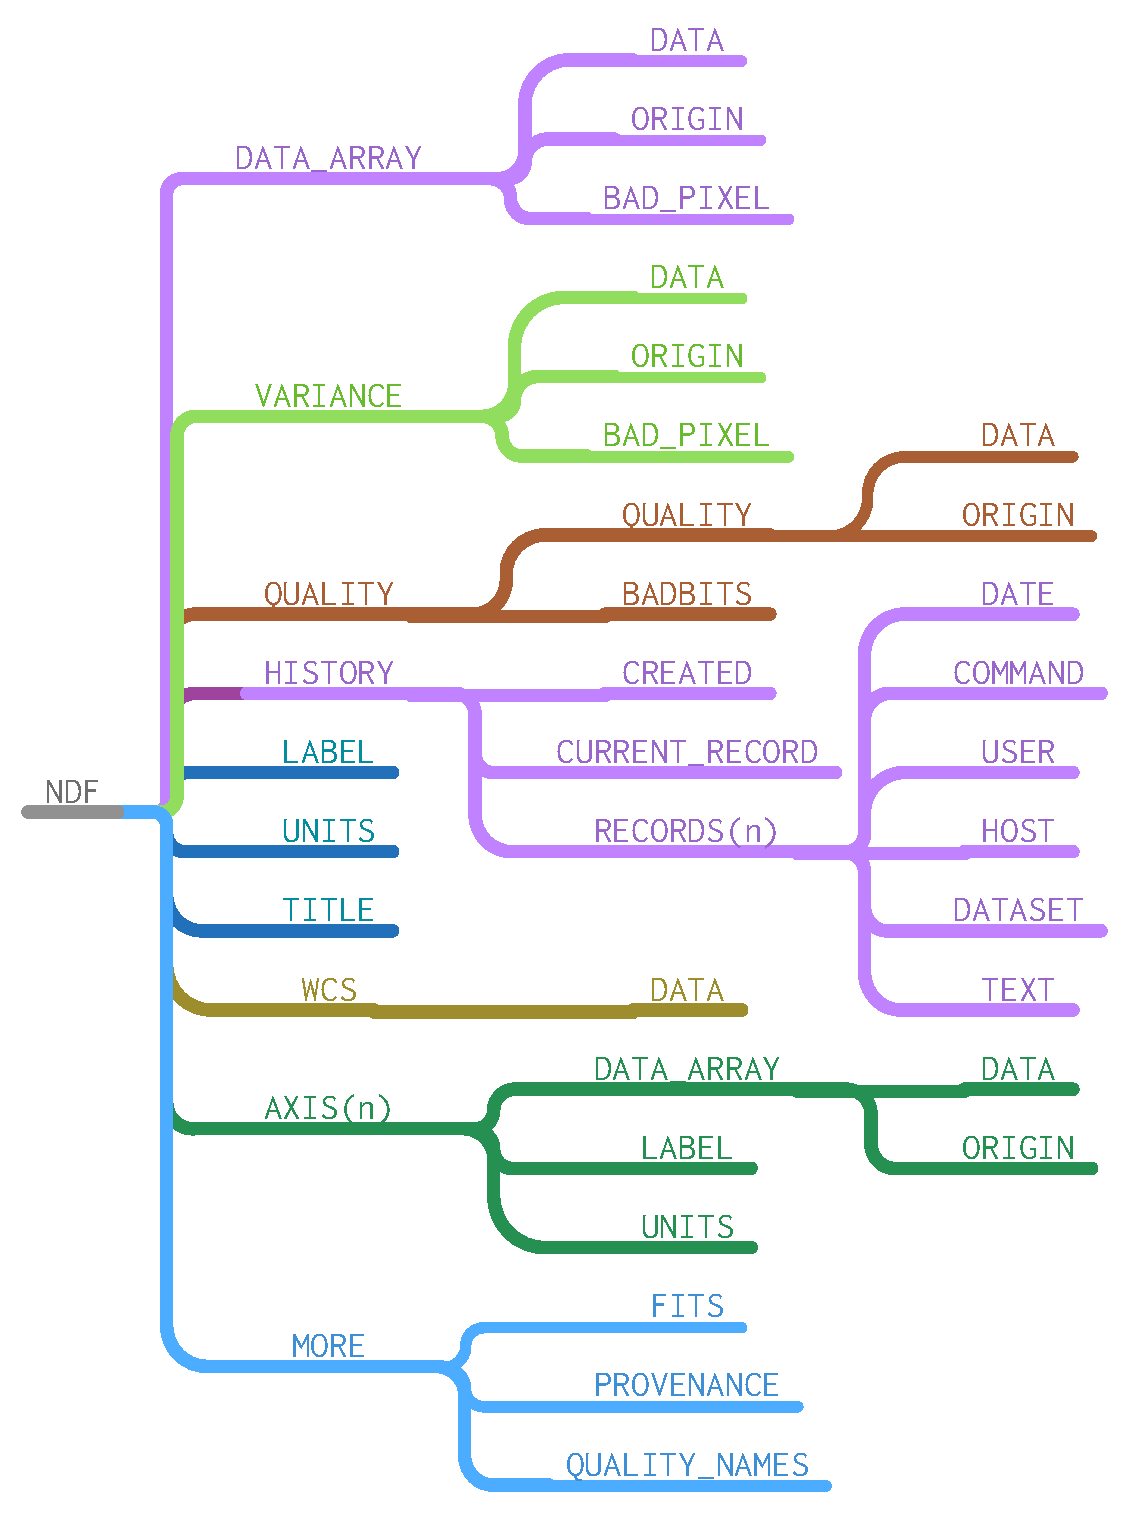
\includegraphics[width=\columnwidth]{NDF-structure}
\caption{Schematic of the NDF hierarchy. All components are optional
  except for \texttt{DATA\_ARRAY}.}
\label{fig:ndf-structure}
\end{figure}

Given the situation with competing schemes for using the hierarchy, it
become clear that a unified data model was required. A working group
was formed to analyze the competing models and come up with a standard and this work
was completed in the late 1980s \citep{1988STARB...2...11C,SGP38}.
After much debate it was decided to develop a data model that included
the minimum structures to be useful for the general astronomer without
attempting to be everything to everybody but designing in an extension
facility from the beginning. The resulting model was named the
extensible \emph{N}-Dimensional Data Format (NDF).  NDF combined some
features of the \emph{IMAGE} scheme, such as the use of
\texttt{DATA\_ARRAY}, and some features adopted from Asterix, from
which the \texttt{HISTORY} structure was adopted complete.  The
decision to recognize NDF structures based on the presence of a
\texttt{DATA\_ARRAY} array was an important compromise as it allowed
data in the \emph{IMAGE} format, which indirectly included data in
BDF format that had been converted previously, to be used immediately
in applications that had been ported to use the NDF library.

In the following sections we describe the core components of the NDF
data model to provide an overview of the NDF approach concerning what
is covered by the model and what is deliberately left out of the
model. For more details on NDF please see the detailed NDF design
document \citep[SGP/38;][]{SGP38} and library documentation \citep[SUN/33;][]{SUN33}.

\subsection{Data Arrays}

NDF supports the concept of a primary data array and an associated
variance array and quality mask. Variance was selected as the error
component to reduce the computational overhead when propagating errors
during processing. All three components share the same
basic \texttt{ARRAY} structure which defines the dimensionality of the
array and allows for the concept of a pixel origin. The
\texttt{BAD\_PIXEL} flag is intended as a hint to application
software to allow simpler and faster algorithms to be used if it is known
that no bad values are present in the data array. Additionally, the flag
can be used to indicate that all values are to be used, thereby
disabling bad value handling and allowing the full range of a data
type. This was felt to be particularly important for the shorter
integer data types.

{\small
\begin{verbatim}
DATA_ARRAY     <ARRAY>         {structure}
  ORIGIN(2)      <_INTEGER>      2,2
  DATA(300,300)  <_REAL>         0.0598,0.0237
                                 ... 0.2154, 0.0234
  BAD_PIXEL      <_LOGICAL>      FALSE

VARIANCE       <ARRAY>         {structure}
  ORIGIN(2)      <_INTEGER>      2,2
  DATA(300,300)  <_DOUBLE>       *,*,*,*,*,*,*,
                                 ... *,*,*,*,*
\end{verbatim}
}

The quality mask uses the \texttt{ARRAY} type but includes an extra
level in the structure to support a bit mask. The \texttt{BADBITS}
mask can be used to enable or disable planes in the \texttt{QUALITY} array.

{\small
\begin{verbatim}
QUALITY        <QUALITY>       {structure}
  QUALITY        <ARRAY>         {structure}
    ORIGIN(2)      <_INTEGER>      2,2
    DATA(300,300)  <_UBYTE>      3,3,3,3,3,3,
                                   ... 3,3,3,3

  BADBITS        <_UBYTE>        32
\end{verbatim}
}

For applications that do not wish to support explicit quality tracking
the NDF library supports the ability to automatically mask the data
and variance arrays based on the mask, setting the corresponding value
in the variance array to a magic value when the data are mapped into
memory. Unlike the \emph{IMAGE} scheme
or FITS, which allow the magic (or blank) value to be specified per
data array, NDF specifies the magic value to be used for each data type
covering both floating point and integer representations, inheriting
the definition from the underlying HDS definition. Indeed,
\texttt{NaN} is not explicitly part of the standard and it is usually
best to convert \texttt{NaN} elements to the corresponding floating point magic
value before further processing is applied. A single definition of the
magic value for each data type simplifies applications programming and
removes the need for the additional overhead of providing a value for
every primitive data array.

\texttt{NaN} was excluded from the standard as it was not
supported in VAX floating point \citep[see e.g.][]{660194} and the Starlink
software was not ported to machines supporting IEEE floating point
until the 1990s \citep[e.g.,][]{1991STARB...8...11C}. Unlike FITS, which
did not officially support floating point until 1990
\citep{1989FPFITS,1991BAAS...23..993S} when they were able to adopt
\texttt{NaN} as part of the standard, much software pre-existed in the
Starlink environment by this time and it was decided to continue with
the magic value concept rather than attempt to support multiple magic
values in floating point data.

\subsubsection{Data compression}

The original NDF standard included the \emph{SCALED} data compression
variant, which is commonly required when representing floating point numbers in
integer form; this is equivalent to \texttt{BSCALE} and \texttt{BZERO} in
FITS, although this variant was not implemented in the NDF library
until 2006 \citep{2008ASPC..394..650C}. In 2010 a lossless delta
compression system for integers was added to support raw SCUBA-2 data
\citep{2013MNRAS.430.2513H}. This was a new implementation of the
\texttt{slim} data compression
algorithm\footnote{\url{http://sourceforge.net/projects/slimdata/}}
developed for the Atacama Cosmology Telescope
\citep{2004SPIE.5498....1F}.

\subsection{Character Attributes}

Each NDF has three character attributes that can be specified: a
title, a data label and a data unit. These values can be accessed
through the library API without resorting to a FITS-style extension.

\subsection{Axes and World Coordinate Systems (WCS)}

Axis information was initially specified using an \texttt{AXIS} array
structure with an element for each dimension of the primary data
array. The axis information was specified in an \texttt{ARRAY} type
structure as for data and variance and allowed axis labels and units
to be specified. For each axis, coordinates were specified for each
pixel in the corresponding dimension of the data array. This allowed
for non-linear axes to be specified and is similar to the
\texttt{-TAB} formalism later adopted in FITS \citep{2006A&A...446..747G}.

{\small
\begin{verbatim}
AXIS(3)      <AXIS>       {array of structures}

Contents of AXIS(1)
  DATA_ARRAY   <ARRAY>      {structure}
    ORIGIN(1)    <_INTEGER>   -74
    DATA(187)    <_DOUBLE>    0.041666,0.0411111,
                              ... -0.061666

  LABEL        <_CHAR*22>   'Right ascension offset'
  UNITS        <_CHAR*3>    'deg'
\end{verbatim}
}

The \texttt{AXIS} formalism worked well for spectral coordinates but
it did not solve the general problem of coupled coordinates such as
Right Ascension and Declination or how to change the representation of
an axis, for example when changing from wavelength to frequency or from
ICRS to Galactic. A more general solution was required and this
prompted the development of the AST library
\citep{1998ASPC..145...41W} with an object-oriented approach to
generalised coordinate frames. AST support was added to the NDF
standard in 2000 \citep{2001ASPC..238..129B} by adding a new top-level
\texttt{WCS} structure to NDF.

{\small
\begin{verbatim}
WCS        <WCS>    {structure}
  DATA(229) <_CHAR*32> 'Begin FrameSet','Nframe = 5',
                   ... ' End CmpMap',' End FrameSet'
\end{verbatim}
}

AST objects were stored simply as an array of strings using the native
ASCII representation. The library API was modified to support routines
for reading and writing AST objects without the library user knowing
how the object is represented in the hierarchical model.

The NDF library manages a number of WCS frames specifically intended to
describe coordinate systems defined by the NDF library:

\begin{description}
\item[\texttt{GRID}] - a coordinate frame in which the first pixel in the NDF is
centred at coordinate (1,1). This is the same as the ``pixel coordinate
system'' in FITS.
\item[\texttt{PIXEL}] - a coordinate frame in which (0,0) corresponds to
the pixel origin of the NDF. The transformation between \texttt{PIXEL}
and \texttt{GRID} is a simple shift of origin.
\item[\texttt{AXIS}] - a coordinate frame that corresponds to AXIS
structures (if any) stored in the NDF.
\item[\texttt{FRACTION}] - a coordinate frame in which the NDF spans a
unit box on all pixel axes.
\end{description}

The NDF library always removes the above frames when storing the
collection of WCS frames
within an NDF, and re-creates them using the current state of the NDF
when returning a FrameSet for an NDF.

\subsection{History}

The \texttt{HISTORY} structure is used to track processing history and
includes the date, application name, arguments and a narrative
description. The structure was first developed for the
\asterix\ application and adopted directly into the NDF data
model. The history was intended specifically to not be parseable by
application software but applications such as SURF
\citep{1998ASPC..145..216J} did use the history to determine whether a
particular application had been run on the data so the user could be
informed if they have missed a mandatory step in the processing.

{\small
\begin{verbatim}
HISTORY        <HISTORY>      {structure}
  CREATED        <_CHAR*24>   '2014-FEB-04 23:40:26.412'
  CURRENT_RECORD  <_INTEGER>  2
  RECORDS(10)    <HIST_REC>   {array of structures}

  Contents of RECORDS(1)
   DATE        <_CHAR*24>   '2014-FEB-04 23:40:28.153'
   COMMAND     <_CHAR*30>   'MAKEMAP (SMURF V1.5.0)'
   USER        <_CHAR*4>    'user'
   HOST        <_CHAR*13>   'host.io'
   DATASET     <_CHAR*30>   '/data/results.sdf'
   TEXT(78)    <_CHAR*72>   'Parameters: BBM=FALSE',
                            ... 'REFRES=3.0"'
\end{verbatim}
}

Comparing the above trace to that shown in Fig.~\ref{fig:asterix},
the only change involves the increase in resolution of the time
stamp to support milliseconds. This was required as computers have
become faster over the years and many processing steps can occur
within a single second. Provenance handling, \S\ref{sec:provenance},
uses the history block to disambiguate provenance entries and relies
on the timestamp field.

\subsection{Extensions}

The NDF standard included a special place, named \texttt{MORE}, for local extensions to the
model. This allowed instruments and applications to track additional
information without requiring standardisation. The only rule was that
each extension should be given a reserved name and that the data type
would define the specific data model of an extension. Some
applications, for example, went so far as to include covariance
information in extensions to overcome limitations in the default error
propagation model for NDF \citep[for example \specdre;][]{SUN140}.

Three extensions proved so popular that they are now effectively part of the NDF
standard, but for backwards compatibility with existing usage they can
not be moved out of the extension component.

\subsubsection{FITS headers}

FITS headers, consisting of 80-character header cards, are extremely
common and to simplify interoperability with FITS files and to
minimize structure overhead, as was found from experience with DST,
it became commonplace to store the header \emph{as is}
as an array of 80-character strings matching the FITS
convention rather than attempting to parse the contents and expand
into structures.

\subsubsection{Provenance}
\label{sec:provenance}

\begin{figure}
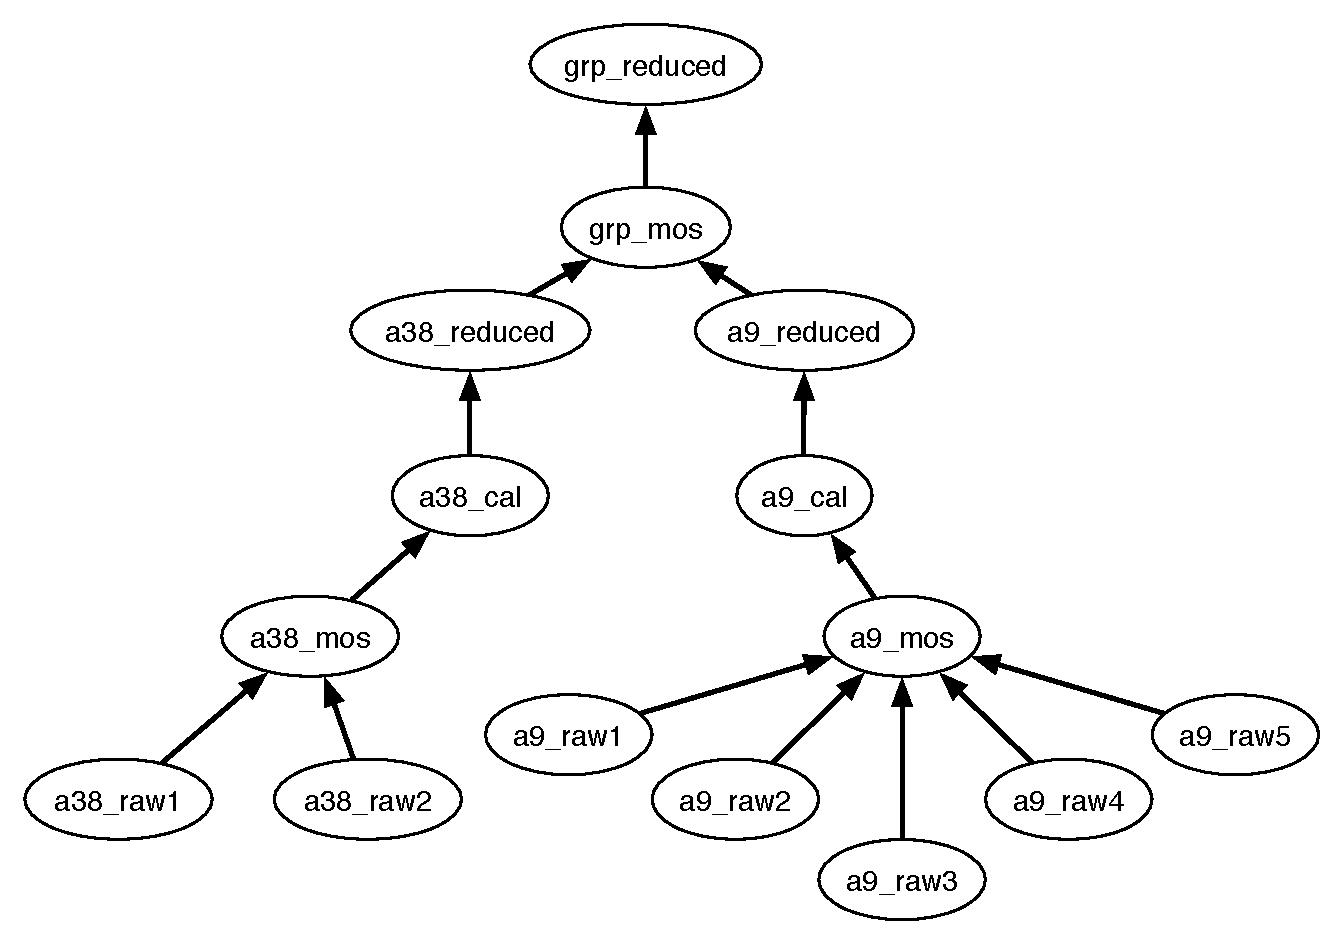
\includegraphics[width=\columnwidth]{provenance.pdf}
\caption{A simple provenance tree for an example of two observations
  being reduced independently and then co-added into a final
  mosaic.}
\label{fig:prov}
\end{figure}

In the late 1980s disk space and processing power were more highly
constrained than they are now. At the time therefore, it
seemed prudent to limit history propagation to a single ``primary''
parent.  As a consequence the NDF library ensures that each application
copies history information from a single primary parent NDF to each
output NDF, appending a new history record to describe the new
application. This means that if many NDFs are combined together by a
network of applications, then each resulting output NDF will, in
general, contain only a subset of the history needed to determine all
the NDFs and applications that were used to create the NDF. It would
of course be possible to gather this information by back-tracking
through all the intermediate NDFs, analysing the history component of
each one, but this depends on the intermediate NDFs still being
available, which is often not the case.

In 2009, it was decided that the inconvenience of this ``single line of
descent'' approach to history was no longer justified by the savings in
disk space and processing time, and so an alternative system was
provided that enables each NDF to retain full information about all
ancestor NDFs, and the processing that was used to create them \citep{2009ASPC..411..418J,2011tfa..confE..42J}. Thus
each NDF may now contain a full ``family tree'' that goes back as far as
any NDFs that have no recorded parents, or which have been marked
explicitly as ``root'' NDFs. Each node in the tree records the name of
the ancestor NDF, the command that was used to create it, the date and
time at which it was created, and its immediate parent nodes. Each
node also allows arbitrary extra information to be associated with the
ancestor NDF. Care is taken to merge nodes -- possibly inherited from
different input NDFs -- that refer to the same ancestor. A simple
provenance tree is shown in Fig.~\ref{fig:prov}.

For reasons of backward compatibility, it was decided to retain the
original NDF History mechanism, and add this new ``family tree''
feature as an extra facility named ``Provenance''.  Originally the
family tree was stored as a fully hierarchical structure within an NDF
extension, using raw HDS. However, given the possibility for
exponential growth in the number of ancestors, the cost of navigating
such a complex structure quickly became prohibitive. Therefore,
storage as raw HDS was replaced by an optimised bespoke binary format
packed into an array of integers (the provenance model is outlined in
\ref{app:prov}).

\subsubsection{Quality Labels}

Individual bits in the quality mask can be addressed using the
\texttt{BADBITS} attribute but the NDF standard did not allow for
these bits to be labeled. This confusion was solved first in the
\iras\ package which added a \texttt{QUALITY\_NAMES}
extension associating names with bits. \KAPPA\ tasks were then
modified to understand this convention and allow users to enable and
disable masks by name.

\subsection{Library Features}

Above and beyond the core data model, the NDF library provides some
additional features that can simplify application development. The
library uses very much an object-oriented interface, despite being
developed in Fortran and the python interface, \texttt{pyndf}, provides a full object
interface whereby an NDF object can have methods invoked upon it and
provides direct access to object attributes such as dimensionality and
data label.

\subsubsection{Component Propagation}

The default behavior of the NDF library encourages the convention
that all applications should copy any unrecognised extensions
unchanged from input to output. Applications are free to modify this
default behaviour, but in general do not do so.

\subsubsection{Slicing}

The NDF library allows a subset of the array to be selected using a
slicing syntax that can work with variety of coordinate systems. The
user can specify the section in pixel coordinates (where the pixel
origin is taken into account) or in world coordinates, either in the
legacy \texttt{AXIS} scheme or using full WCS support. The section can
either be specified using bounds or a center coordinate and
extent. Example sections are
\begin{verbatim}
myimage(12h59m49s~4.5m,27.5d:28d29.8m)
\end{verbatim}
to extract an area from an image where the Right Ascension is
specified as a radius and the Declination using bounds;
\begin{verbatim}
myspectrum(400.:600.)
\end{verbatim}
where the spectrum is truncated to a range of, say, 400 to 600\,km/s;
\begin{verbatim}
mycube(12h34m56.7s,-41d52m09s,-100.0:250.0)
\end{verbatim}
where a spectrum is extracted from a cube at a particular location and
also truncated;
\begin{verbatim}
mycube(55:63,75~10,-100.0:250.0)
\end{verbatim}
where a subset of a cube is extracted where the first two coordinates
specify pixel bounds and the third coordinate is a world coordinate range.

\subsubsection{Chunking \& Blocking}

Mapping large data arrays into memory can use considerable resources
and astronomical data always seems to be growing at a rate slightly
exceeding the computers available to the average astronomer. The NDF
library provides an API to allow subsets of a data array to be mapped
in chunks to allow data files to be processed in smaller pieces. The
concept of blocking is also used to allow a subset of the image to be
mapped in chunks of a specified dimension. The distinction between
chunking and blocking is significant in that chunking returns the data
in sections that are contiguous in memory for maximum efficiency
whereas blocking allows spatially related pixel data to be returned at
the expense of performance for reordering the data array.

\subsubsection{Foreign Format Conversion}

The NDF format has always been one format amongst many formats in astronomy and much work has been
expended on providing facilities to convert NDF files into FITS and
IRAF format and convert from those formats into NDF \citep{SUN55}. In
many cases an astronomer would like to use a particular NDF
application on a FITS file without realising that the application does
not natively support FITS. If foreign format conversion is enabled the
NDF library will run the appropriate conversion utility based on the
file suffix and present the temporary file to the application. If the
user specifies an output file with a particular foreign format suffix
the NDF library will create a temporary NDF for the output and convert
it when the file is closed.

\subsubsection{Automated History}

The library API was designed to make history updating as easy
as possible and by default if the history structure existed the NDF
library automatically adds a new entry when a file was written
to.

\subsubsection{Event Triggers}

Callback routines can be registered to be called in response to files
being read from, written to, opened or closed. This facility is used
by the NDG library \citep{SUN2} to enable provenance handling
as a plugin without requiring direct changes to the NDF library itself.

\section{Data Acquisition}
\label{sec:daq}

Figaro had a strong influence on the infrared spectroscopy community
in the United Kingdom and the United Kingdom Infrared Telescope
(UKIRT) adopted the DST format for CGS3 and CGS4 \citep{1993SPIE.1946..547W}. NDF was adopted in
1995 although each instrument had a slightly different flavor of
metadata and handling of multiple exposures involved distinct data
files. A unified UKIRT NDF format for all instruments, involving HDS
containers of NDF structures to handle multiple exposures, was
adopted with the release of the ORAC system \citep{2000SPIE.4009..227B}.

The James Clerk Maxwell Telescope (JCMT) initially used a proposed
submillimeter standard format known as the Global Section Datafile
\citep[GSD;][formerly General Single Dish Data]{sun229}. In 1996 SCUBA
\citep{1999MNRAS.303..659H} was delivered using the NDF format and a
unified NDF raw data format was adopted for ACSIS
\citep{2009MNRAS.399.1026B} from 2006 and SCUBA-2
\citep{2013MNRAS.430.2513H} from 2009.

The Anglo-Australian Observatory (AAO) adopted HDS and initially used
the DST format for instruments such as UCLES
\citep{1990SPIE.1235..562D}. IRIS \citep{1993PASAu..10..298A} could
use both DST and NDF format, whereas 2DF \citep{2002MNRAS.333..279L}
used NDF.

\section{Lessons Learned}
\label{sec:lessons}

For a variety of reasons, the Starlink software, and hence the NDF
format, did not receive much traction outside the UK, particularly in
the US astronomical community that closely adhered to FITS until the
advent of HDF. This is regrettable as NDF proved to be a rich and
flexible data format that has aged well against mounting requirements
from data processing environments. Perhaps the ultimate lesson learnt
is that data formats are adopted and retained for sociological reasons
as much as for technical reasons.

\subsection{Key Successes}
\label{sec:success}

{\color{red}Need introductory remarks. NXG: \emph{What we got right
    and what you should carefully consider}. Maybe remove subsections
  and simply have introduction, bullets, detailed
  explanation. Recapitulate what happened without these
  features. Include difficulties with marketing a new format? Although
that isn't really a \emph{key success}.}

\subsubsection{Hierarchy can be useful}

Initially it was very hard to convince people that hierarchical data
structures were at all useful. This can be seen in the Wright-Giddings
layout of a simple astronomical image file using HDS. Over the years
the adoption of hierarchy has been an important part of the NDF
experience. The ability to relocate or modify parts of a data file,
changing the organization, or to copy related sections to a new file
is very powerful.  NDF extensions containing NDF structures, allowing
software packages to extract those NDFs or simply focus on them
without regard to the enclosing data module becomes very intuitive and
obvious once it is learned. A flat layout would require additional
grouping metadata to understand which components were related and this
is neatly handled by a simple hierarchy.

\subsubsection{Do not try to do everything}

There are two incompatible approaches to designing a data model. The
default position tends to be to think of everything that is needed for
all of astronomy and try to design a model where all metadata is
described and everything has its place. This is the approach taken by
the IVOA \citep[see e.g.][]{2012arXiv1204.3055M} and leads to long and
heated discussions that generate data models that are never quite
perfect and continually need to be tweaked as new instrumentation and
metadata are developed. This is a worthy goal and it is clear that
much can be gained if these data models can be utilised, especially if
related models (spectrum and image when combined into a data cube)
share common ground.

For NDF there was a need to generate a usable model quickly that took
concepts that were generically useful, leaving instrumental details to
extensions. These extensions were ignored by generic software packages
although clear rules were made regarding how extensions should be
propagated. This approach allowed for the format to grow without
requiring the format or the NDF library to understand the
contents of extensions.

This approach has been very successful, not only in enabling new
features to be added to NDF once the need became obvious, but also
in so far that wavelength regimes not initially involved in the
discussion can make use of NDF without requiring that the core data
model be changed.

\subsubsection{Standardised features aid application writers}

Once application writers understand that there is a standard place for
error information, quality masks and other features of the standard
data model, they begin to write application software that can use
these features. Not having to use a heuristic to determine whether a
particular data array represents an image or an error can allow the
application writer to focus more on the algorithms that matter. Once
users of the software understand that errors and masks are an option
they begin to have an expectation that all the software packages will
handle them. This then motivates the developer to support these
features.  This is especially true if the core concepts of the data
model are simple enough that the learning curve is small.

\subsection{Other Good Features}

{\color{red}Need to introduce this section}

\subsubsection{Round-tripping to other data formats}

For a new format to be used it must be possible to
convert to and from existing formats in a safe and reliable manner
without losing information.
Significant effort was spent in developing conversion software that
would allow conversion to and from NDF
\citep{SUN55,1997STARB..19...14C}. In particular, special code was
used to recognize specific data models present in FITS files to enable
a more accurate conversion of scientific information into the NDF
form. Support was also added for the \emph{multispec} format in IRAF
\citep{1993ASPC...52..467V} to ensure that wavelength scales were not
lost.

\subsubsection{Adoption of FITS header}

Given hierarchical structures the default assumption might be to use
arrays of keyword structures where each structure would contain the
value, the comment and the unit. Alternatively simply drop the unit
and comment and just use keyword/value pairs. These approaches turned
out to be extremely slow and space inefficient so a pragmatic solution
was taken to standardise on an array of characters formatted
identically to a FITS header. The initial NDF standard did not include
this approach and parsing of a FITS header is left up to the user
rather than being integral to the NDF library. In practice the AST
library \citep{1998ASPC..145...41W} is often used for processing the FITS
header from an NDF so this causes few problems and simplifies the NDF
organization.

\subsubsection{Structure Data Types}

{\color{red} This needs a better example given that, as it turns out,
  the NDF library doesn't look at the structure type when looking for NDFs.}

The ability to associate a data type with a structure is important for
the ability of applications to know how to process particular
structures. An NDF extension may itself include many more NDF
structures each of which would have a different name but could also
share the data type of \texttt{NDF}. For example, the \gaia\
visualization tool \citep{2009ASPC..411..575D} will scan the HDS file
for all such NDF structures and make them available for
display. Applications can therefore make decisions on how to handle a
structure without having to know its name.

\subsubsection{Proven ability to enhance format}

The initial NDF design document did not profess to know the future and
was deliberately designed to allow new features to be added as they
became necessary. The adoption of a character array matching an
80-character FITS header was an early change but there have also been
changes to support world coordinate objects
\citep{2001ASPC..238..129B}, data compression algorithms
\citep{2008ASPC..394..650C} and provenance tracking
\citep{2009ASPC..411..418J}. The NDF standard is continuing to evolve
to meet the needs of modern astronomy data processing.

NDF combined with HDS was a conscious decision to not develop an
interchange or archive format. HDS was designed solely to be accessed
through a reference implementation library and API and many of the NDF
features were directly integrated into the reference NDF library without being
specified in the core data model.  This yielded great flexibility
regarding exactly how the data are stored and greatly simplified
future enhancemants (and general future-proofing) because changes to
the data format and how data are accessed could all be hidden from
applications by changes made in one place. However, care needs to be taken
when rolling out updates: software linked with old versions
may not be able to read newer data. Indeed, HDS includes an internal
version number and can read earlier versions of the data format, but if a
newer version is encountered than supported by the library HDS will
know about it and report the problem.

\subsection{Areas for improvement}

{\color{red}Need to introduce this section}
As NDF has been used we have come to realise that some parts of the
standard could do with adjustment and other enhancements.

\subsubsection{Quality masking}

The initial design for the quality mask used a single unsigned byte
allowing 8 different quality assignments in a single data file. The
design did not allow for the possibility of supporting larger unsigned
integer data types. This restriction should be raised to allow more
assignments. The SMURF map-maker
\citep[][\ascl{1310.007}]{2013MNRAS.430.2545C} already makes use of more
than 8 internally and uses an unsigned short. When the results are
written out mask types have to be combined if more than 8 were present
in the output data file.

\subsubsection{Table support}

Tables were added to FITS \citep{1988A&AS...73..365H} during the
initial development of NDF and the need for tables got lost in the
drive for a standardised image format. A table type was never added to
NDF and Starlink software eventually took the pragmatic solution of
using FITS binary tables \citep{1995A&AS..113..159C} for output
tables. This cannot solve the problem of integrating data tables into
image data files and the format would benefit from a native data
type. The JCMT raw data format instead uses individual 1-dimensional
data arrays to store time-series data but this is inefficient and adds
programming overhead.

{\color{red} Say how FITS2NDF handles binary tables.}

\subsubsection{Flexible variance definitions}

The adoption of variance as a standard part of NDF was an important
motivator for application writers to add support for error propagation and
almost all the Starlink applications now support variance. The next
step is to support different types of errors, including
covariance \citep[see e.g.][]{1992ESOC...41...47M}. This has been proposed many times \citep[see
e.g.][]{1991STARB...8...19M} but is a very difficult problem to solve
in the general case and may involve having to support pluggable
algorithms for handling special types of error propagation.

\subsubsection{Extension complexity}

Many extensions created in the early years of NDF became more complex
than was strictly necessary by ignoring the design decisions of NDF and
using highly complex HDS structures. In many cases it would have been
beneficial to use NDF structures in the extensions which would have
allowed the NDF library to read the data (by giving the full path to
the structure) without resorting to low-level HDS API calls. The NDF
structures would also have been visible to general purpose tools for
visualization.

\subsubsection{Data checksums}

The FITS \texttt{DATASUM} facility is very useful and NDF should support
it. Ideally it should be possible to generate a reference checksum for
a structure. It may be that this has to be done in conjunction with
HDS.

\subsubsection{Character encodings}

The \texttt{\_CHAR} data type in HDS uses an 8-bit character type,
assumed to be ASCII. It was designed long before Unicode came to exist
and has no support for accented characters or non-ASCII character
sets. Multi-byte Unicode should be supported in any modern format to
allow metadata to be represented properly. HDS can not support the
storage of common astronomical units such as $\upmu$m or $\AA$.
It may be possible to use the automatic type conversion concept
already in use for numeric data types
to allow Unicode to be added to NDF without forcing every application
to be rewritten. If an application uses the standard API for reading character
components they will get ASCII even if that involves replacing Unicode
characters with either normalised versions of characters outside the
ASCII character set (for example, dropping accents) or whitespace. A new API
would be provided for reading and writing Unicode strings.

\subsubsection{Provenance Growth}

Whilst the provenance handling works extremely well and is very useful
for tracking what processing has gone into making a data product, the
provenance information can become extremely large during long and
complicated pipeline processing such as those found in products from
ORAC-DR \citep{2008AN....329..295C}.  There can be many thousands of
provenance entries including some loops where products are fed back
into earlier stages because of iterations.  The provenance tracking
eventually begins to take up a non-trivial amount of time to collate
and copy from input files to output files. One solution to this may be
to offload the provenance handling to a database during processing,
only writing the information to the file when processing is complete
and the file is to be exported. It would be fairly straightforward to
modify the NDG library to use the Core Provenance Library
\citep{Macko:2012:GPL:2342875.2342881}.

\subsubsection{Library limitations}

Whilst there are many advantages to having a single library
providing the access layer to an NDF, there is also a related problem
of limitations in this one library causing limitations to all
users. In particular the current NDF library is single-threaded due to
use of a single block of memory tracking access status. Furthermore
the HDS library itself is also single-threaded with its own internal
state. As more and more programs become multi-threaded to make use of
increased numbers of cores in modern CPUs this limitation becomes more
and more frustrating.

Another issue associated with the library is the use of 32-bit
integers as counters in data arrays. It is now easy to imagine data
cubes that exceed this many pixels and a new API may be needed to ease
the transition to 64-bit counters.

Whilst the HDS library is written entirely in ANSI C, the NDF and
related ARY \citep{SUN11} and NDG \citep{SUN2} libraries are written
mainly in Fortran.
This can cause a reticence to adoption from people outside the Starlink community and
adds complications when providing interfaces to higher-level languages
such as Python, Perl and Java. Indeed a subset of the NDF model  was
written as a Java layer on top of the C HDS library, precisely to
avoid the added dependency to the Fortran runtime library.

Ideally NDF would be rewritten in C and be made thread-safe.

\section{Conclusions}
\label{sec:conclusion}

The NDF data model did bring order to the chaos of arbitrary
hierarchical structures and succeeded in the
promise of providing a base specification that can be adopted by many
applications processing data from disparate instrumentation.

From its beginnings in the mid-1980s the NDF data model has been used
throughout the Starlink software collection within diverse
applications such as \smurf\ \citep{2013MNRAS.430.2545C},
\ccdpack\, \gaia\ and \KAPPA.
It has also been used as a raw data acquisition format at the
Anglo-Australian Observatory, the James Clerk Maxwell Telescope and the United Kingdom Infrared
Telescope and NDF format data are available from
from the UKIRT and JCMT archives at the Canadian Astronomy Data Centre
\citep{2008ASPC..394..450E,P01_adassxxiii}. The shift from arbitrary
use of hierarchical structures to a data model enforced by a library
and API is extremely important.

The NDF data model also supported a number of data-structuring
experiments.
The model allowed applications written in Fortran to
adopt object-oriented methodologies by adopting NDF as a backing store
and using the self-describing features to represent objects
\citep{1993ASPC...52..199B}.
The HDX framework \citep{2003ASPC..295..221G} was developed around 2002 as a flexible
way of layering high-level data structures, presented as a virtual XML
DOM, atop otherwise unstructured external data stores.  This was in
turn used to develop Starlink's NDX framework, which allowed FITS
files to be viewed and manipulated using the concepts of the NDF
format.  The NDX experiment was an attempt to directly apply the
lessons of the long NDF/HDS experience -- namely that a small amount of
structure, overlaid on conceptually separate bitbuckets, can very
promptly bring order out of chaos.
However, there was no take up in the community outside of the Starlink Java applications
such as \treeview\ \citep{2003ASPC..295..445B} and
\splat\ \citep[][\ascl{1402.007}]{2005ASPC..347...22D}.

For the future we are considering the possibility of replacing the HDS
layer with a more widely used hierarchical data format such as HDF5
\citep{Folk:2011:OHT:1966895.1966900}. This would have the advantage
of making NDF available to a much larger community, albeit with NDF
still being in Fortran, and also remove the
need to support HDS in the longer term. NDF and all the existing
Starlink applications would continue to work so long as a conversion
program is made available to convert HDS structures to HDF5 structures.
This would have the added advantage of making it straightforward to
add support for tables natively to the NDF data model. Many of the
concepts in NDF map directly to HDF5. One remaining issue is that HDF5
does not support the notion of arrays of groups so the
\texttt{HISTORY} and \texttt{AXIS} structures in NDF would need to be
remapped into a flatter layout, maybe with numbered components in an
\texttt{AXIS} or \texttt{HISTORY} group.

\section{Acknowledgments}

This research has made use of NASA's Astrophysics Data System.
The Starlink software is currently maintained by the Joint Astronomy
Centre, Hawaii with support from the UK Science and Technology
Facilities Council. We thank Jim Peden and Trevor Ponman for providing
comments on the manuscript regarding the early days of HDS and the
development of \asterix.

The source code for the NDF library and the Starlink software
(\ascl{1110.012}) is open-source and is available on Github at
\htmladdnormallink{https://github.com/Starlink}.

%% The Appendices part is started with the command \appendix;
%% appendix sections are then done as normal sections

\appendix

\section{The Provenance Data Model}
\label{app:prov}
This appendix describe the data model used to record the ``family tree'' of
ancestor NDFs that were used to create an NDF. Each node in the tree
describes a single NDF, with the root node being the NDF for which
provenance is being recorded. Thus the parents of the root node each
describe one of the NDFs that were used to create the NDF described by the
root node. A node stores the following items of information about the
associated NDF:

\begin{itemize}
\item The path to the NDF within the local file system. This is a blank
string for the root node, since the main NDF may be moved to a new location.
\item The UTC date and time at which the NDF was created.
\item A boolean flag indicating if the NDF is ``hidden'' - meaning that
the NDF will not be included as an ancestor when provenance is copied
from one NDF to another.
\item A string identifying the command that created the NDF.
\item History information. For the root node, this is just a 4-byte hash code
that represents the contents of the main NDF's History component. This hash
code is subsequently to identify the same history information within other
NDFs. For non-root nodes, the history information contains any history
records read from the corresponding ancestor NDF that were not also present
in any of the ancestors direct parents\footnote{This is done to avoid unnecessary
duplication of History records in different Prov structures.}.
\item Any extra arbitrary information associated with the NDF. There are no conventions on what this extra information
represents.
\item A list of pointers to nodes representing the direct parents of the
NDF.
\end{itemize}

The full tree of nodes is stored on disk in an extension named
\texttt{PROVENANCE} within the main NDF, and is encoded into an array of
integers in order to avoid the overhead of reading and writing complex
HDS structures.

Each application will normally first create a basic tree for each output
NDF, holding a single root node describing the output NDF. It will then
read the provenance tree from each input NDF and append each one to the
provenance tree of the output NDF, making it a direct parent of the root
node. When the application closes, the final output tree is stored in
the output NDF.

This whole process can be automated by registering handlers with the NDF
library that are called whenever an NDF is opened. The only change that
then needs to be made to an application to enable basic provenance tracking is for the
application to add two calls to mark the start and end of a ``provenance
recording context''. Alternatively, to achieve finer control of which
input NDFs are recorded as parents of each output NDF, it is possible for
an appliction to handle the reading and writing of provenance trees
itself.

It is possible that a single input NDF may be used many times in the
creaton of an output NDF. For instance, if NDF \emph{A} is added to NDF
\emph{B} to create NDF \emph{C}, and \emph{A} is then added to \emph{C} to create
\emph{D}, then \emph{A} (and all its ancestors) would appear twice in the
provenance tree of \emph{D}. To avoid this, whenever a new parent is added to
the root node, each node within the tree of the new parent is compared to
each node already in the tree. If they match, the tree of the new parent
is ``snipped'' at that point to exclude the duplicated node (and all its
parent nodes). This comparison needs to be done carefully since it is
possible for two nodes to include the same path, creator and date, and
yet still refer to different NDFs\footnote{For instance, if an NDF is
created, used once, and then immediately replaced with a new NDF}. For
this reason, the comparison two nodes are considered equal if:

\begin{enumerate}
\item they have the same path, date and creator, and
\item they have the same number of parent nodes, and
\item each pair of corresponding parent nodes are equal
\end{enumerate}

The third requirement above means that two nodes will never be considered
equal if any of the ancestors of the two nodes differ.




%% References
%%
%% Following citation commands can be used in the body text:
%%
%%  \citet{key}  ==>>  Jones et al. (1990)
%%  \citep{key}  ==>>  (Jones et al., 1990)
%%
%% Multiple citations as normal:
%% \citep{key1,key2}         ==>> (Jones et al., 1990; Smith, 1989)
%%                            or  (Jones et al., 1990, 1991)
%%                            or  (Jones et al., 1990a,b)
%% \cite{key} is the equivalent of \citet{key} in author-year mode
%%
%% Full author lists may be forced with \citet* or \citep*, e.g.
%%   \citep*{key}            ==>> (Jones, Baker, and Williams, 1990)
%%
%% Optional notes as:
%%   \citep[chap. 2]{key}    ==>> (Jones et al., 1990, chap. 2)
%%   \citep[e.g.,][]{key}    ==>> (e.g., Jones et al., 1990)
%%   \citep[see][pg. 34]{key}==>> (see Jones et al., 1990, pg. 34)
%%  (Note: in standard LaTeX, only one note is allowed, after the ref.
%%   Here, one note is like the standard, two make pre- and post-notes.)
%%
%%   \citealt{key}          ==>> Jones et al. 1990
%%   \citealt*{key}         ==>> Jones, Baker, and Williams 1990
%%   \citealp{key}          ==>> Jones et al., 1990
%%   \citealp*{key}         ==>> Jones, Baker, and Williams, 1990
%%
%% Additional citation possibilities
%%   \citeauthor{key}       ==>> Jones et al.
%%   \citeauthor*{key}      ==>> Jones, Baker, and Williams
%%   \citeyear{key}         ==>> 1990
%%   \citeyearpar{key}      ==>> (1990)
%%   \citetext{priv. comm.} ==>> (priv. comm.)
%%   \citenum{key}          ==>> 11 [non-superscripted]
%% Note: full author lists depends on whether the bib style supports them;
%%       if not, the abbreviated list is printed even when full requested.
%%
%% For names like della Robbia at the start of a sentence, use
%%   \Citet{dRob98}         ==>> Della Robbia (1998)
%%   \Citep{dRob98}         ==>> (Della Robbia, 1998)
%%   \Citeauthor{dRob98}    ==>> Della Robbia


%% References with bibTeX database:

\bibliographystyle{model2-names-astronomy}
\bibliography{acndf}

%% Authors are advised to submit their bibtex database files. They are
%% requested to list a bibtex style file in the manuscript if they do
%% not want to use model2-names.bst.

%% References without bibTeX database:

% \begin{thebibliography}{00}

%% \bibitem must have one of the following forms:
%%   \bibitem[Jones et al.(1990)]{key}...
%%   \bibitem[Jones et al.(1990)Jones, Baker, and Williams]{key}...
%%   \bibitem[Jones et al., 1990]{key}...
%%   \bibitem[\protect\citeauthoryear{Jones, Baker, and Williams}{Jones
%%       et al.}{1990}]{key}...
%%   \bibitem[\protect\citeauthoryear{Jones et al.}{1990}]{key}...
%%   \bibitem[\protect\astroncite{Jones et al.}{1990}]{key}...
%%   \bibitem[\protect\citename{Jones et al., }1990]{key}...
%%   \harvarditem[Jones et al.]{Jones, Baker, and Williams}{1990}{key}...
%%

% \bibitem[ ()]{}

% \end{thebibliography}

\end{document}

%%
%% End of file `elsarticle-template-2-harv.tex'.
